\documentclass[portrait,final,a0paper,fontscale=0.285]{baposter}

\usepackage{calc}
\usepackage{graphicx}
\usepackage{amsmath}
\usepackage{amssymb}
%\usepackage{relsize}
\usepackage{multirow}
\usepackage{rotating}
\usepackage{bm}
\usepackage{url}

\usepackage{graphicx}
\usepackage{multicol}
\usepackage{color}

%\usepackage{times}
%\usepackage{helvet}
%\usepackage{bookman}
\usepackage{palatino}
\usepackage{tensor}
\usepackage{etoolbox}
\newtoggle{portrait}
\toggletrue{portrait}

\providecommand{\e}[1]{\ensuremath{10^{#1}}}
\newcommand{\captionfont}{\footnotesize}

%\graphicspath{{images/}{../images/}}
\usetikzlibrary{calc}

\newcommand{\SET}[1]  {\ensuremath{\mathcal{#1}}}
\newcommand{\MAT}[1]  {\ensuremath{\boldsymbol{#1}}}
\newcommand{\VEC}[1]  {\ensuremath{\boldsymbol{#1}}}
\newcommand{\Video}{\SET{V}}
\newcommand{\video}{\VEC{f}}
\newcommand{\track}{x}
\newcommand{\Track}{\SET T}
\newcommand{\LMs}{\SET L}
\newcommand{\lm}{l}
\newcommand{\PosE}{\SET P}
\newcommand{\posE}{\VEC p}
\newcommand{\negE}{\VEC n}
\newcommand{\NegE}{\SET N}
\newcommand{\Occluded}{\SET O}
\newcommand{\occluded}{o}

%%%%%%%%%%%%%%%%%%%%%%%%%%%%%%%%%%%%%%%%%%%%%%%%%%%%%%%%%%%%%%%%%%%%%%%%%%%%%%%%
%%%% Some math symbols used in the text
%%%%%%%%%%%%%%%%%%%%%%%%%%%%%%%%%%%%%%%%%%%%%%%%%%%%%%%%%%%%%%%%%%%%%%%%%%%%%%%%

%%%%%%%%%%%%%%%%%%%%%%%%%%%%%%%%%%%%%%%%%%%%%%%%%%%%%%%%%%%%%%%%%%%%%%%%%%%%%%%%
% Multicol Settings
%%%%%%%%%%%%%%%%%%%%%%%%%%%%%%%%%%%%%%%%%%%%%%%%%%%%%%%%%%%%%%%%%%%%%%%%%%%%%%%%
\setlength{\columnsep}{1.5em}
\setlength{\columnseprule}{0mm}

%%%%%%%%%%%%%%%%%%%%%%%%%%%%%%%%%%%%%%%%%%%%%%%%%%%%%%%%%%%%%%%%%%%%%%%%%%%%%%%%
% Save space in lists. Use this after the opening of the list
%%%%%%%%%%%%%%%%%%%%%%%%%%%%%%%%%%%%%%%%%%%%%%%%%%%%%%%%%%%%%%%%%%%%%%%%%%%%%%%%
\newcommand{\compresslist}{%
\setlength{\itemsep}{1pt}%
\setlength{\parskip}{0pt}%
\setlength{\parsep}{0pt}%
}

%%%%%%%%%%%%%%%%%%%%%%%%%%%%%%%%%%%%%%%%%%%%%%%%%%%%%%%%%%%%%%%%%%%%%%%%%%%%%%
%%% Begin of Document
%%%%%%%%%%%%%%%%%%%%%%%%%%%%%%%%%%%%%%%%%%%%%%%%%%%%%%%%%%%%%%%%%%%%%%%%%%%%%%

\begin{document}

%%%%%%%%%%%%%%%%%%%%%%%%%%%%%%%%%%%%%%%%%%%%%%%%%%%%%%%%%%%%%%%%%%%%%%%%%%%%%%
%%% Here starts the poster
%%%---------------------------------------------------------------------------
%%% Format it to your taste with the options
%%%%%%%%%%%%%%%%%%%%%%%%%%%%%%%%%%%%%%%%%%%%%%%%%%%%%%%%%%%%%%%%%%%%%%%%%%%%%%
% Define some colors

%\definecolor{lightblue}{cmyk}{0.83,0.24,0,0.12}
\definecolor{lightblue}{rgb}{0.05,0.66,1}
\definecolor{mblue}{rgb}{0.0,0.33,0.9}

% Draw a video
\newlength{\FSZ}
\newcommand{\drawvideo}[3]{% [0 0.25 0.5 0.75 1 1.25 1.5]
   \noindent\pgfmathsetlength{\FSZ}{\linewidth/#2}
   \begin{tikzpicture}[outer sep=0pt,inner sep=0pt,x=\FSZ,y=\FSZ]
   \draw[color=lightblue!50!black] (0,0) node[outer sep=0pt,inner sep=0pt,text width=\linewidth,minimum height=0] (video) {\noindent#3};
   \path [fill=lightblue!50!black,line width=0pt]
     (video.north west) rectangle ([yshift=\FSZ] video.north east)
    \foreach \x in {1,2,...,#2} {
      {[rounded corners=0.6] ($(video.north west)+(-0.7,0.8)+(\x,0)$) rectangle +(0.4,-0.6)}
    }
;
   \path [fill=lightblue!50!black,line width=0pt]
     ([yshift=-1\FSZ] video.south west) rectangle (video.south east)
    \foreach \x in {1,2,...,#2} {
      {[rounded corners=0.6] ($(video.south west)+(-0.7,-0.2)+(\x,0)$) rectangle +(0.4,-0.6)}
    }
;
   \foreach \x in {1,...,#1} {
     \draw[color=lightblue!50!black] ([xshift=\x\linewidth/#1] video.north west) -- ([xshift=\x\linewidth/#1] video.south west);
   }
   \foreach \x in {0,#1} {
     \draw[color=lightblue!50!black] ([xshift=\x\linewidth/#1,yshift=1\FSZ] video.north west) -- ([xshift=\x\linewidth/#1,yshift=-1\FSZ] video.south west);
   }
   \end{tikzpicture}
}

\hyphenation{resolution occlusions}
%%
\begin{poster}%
  % Poster Options
  {
  % Show grid to help with alignment
  grid=false,
  % Column spacing
  colspacing=1em,
  % Color style
  bgColorOne=white,
  bgColorTwo=white,
  borderColor=lightblue,
  headerColorOne=mblue,
  headerColorTwo=lightblue,
  headerFontColor=white,
  boxColorOne=white,
  boxColorTwo=lightblue,
  % Format of textbox
  %textborder=roundedleft,
  % Format of text header
  eyecatcher=false,
  headerborder=closed,
  headerheight=0.1\textheight,
%  textfont=\sc, An example of changing the text font
  %headershape=roundedright,
  headershade=shadelr,
  headerfont=\Large\bf\textsc, %Sans Serif
  textfont={\setlength{\parindent}{1.5em}},
  boxshade=plain,
%  background=shade-tb,
  background=plain,
  linewidth=1pt
  }
  % U Logo
  {
\includegraphics[height=3em]{figures/ublogo.jpg}}
  % Title
  {\bf\textsc{Visual Servoing Using Trifocal Tensor}\vspace{0.5em}}
  % Authors
{\textsc{\{ Marwan Osman, Fran\c{c}ois Chaumette \}}\\ \small{University of Burgundy, INRIA Rennes-Bretagne Atlantique and IRISA}} % Author names and institution
  % Technicolor logo
  {% The makebox allows the title to flow into the logo, this is a hack because of the L shaped logo.
    
\includegraphics[height=3em]{figures/ubinrialogo.jpg}
  }

%%%%%%%%%%%%%%%%%%%%%%%%%%%%%%%%%%%%%%%%%%%%%%%%%%%%%%%%%%%%%%%%%%%%%%%%%%%%%%
%%% Now define the boxes that make up the poster
%%%---------------------------------------------------------------------------
%%% Each box has a name and can be placed absolutely or relatively.
%%% The only inconvenience is that you can only specify a relative position
%%% towards an already declared box. So if you have a box attached to the
%%% bottom, one to the top and a third one which should be in between, you
%%% have to specify the top and bottom boxes before you specify the middle
%%% box.
%%%%%%%%%%%%%%%%%%%%%%%%%%%%%%%%%%%%%%%%%%%%%%%%%%%%%%%%%%%%%%%%%%%%%%%%%%%%%%
    %
    % A coloured circle useful as a bullet with an adjustably strong filling
    \newcommand{\colouredcircle}{%
      \tikz{\useasboundingbox (-0.2em,-0.32em) rectangle(0.2em,0.32em); \draw[draw=black,fill=lightblue,line width=0.03em] (0,0) circle(0.18em);}}

%%%%%%%%%%%%%%%%%%%%%%%%%%%%%%%%%%%%%%%%%%%%%%%%%%%%%%%%%%%%%%%%%%%%%%%%%%%%%%
  \headerbox{1. Introduction}{name=definition,column=0,span=2,row=0}{
%%%%%%%%%%%%%%%%%%%%%%%%%%%%%%%%%%%%%%%%%%%%%%%%%%%%%%%%%%%%%%%%%%%%%%%%%%%%%%
      \iftoggle{portrait}{
    \begin{multicols}{2}
  Visual servoing is an approach for controlling the motion of a robotic system from visual measurements \cite{chaumette2006visual}. The trifocal tensor is well known in computer vision for tracing geometric information from three images of the same scene \cite{Hartley2004}.  The trifocal tensor geometric model is more robust than the two view geometry models as it involves the information given by a third view, and the set of correspondences obtained is more robust to outliers.
 {\centering 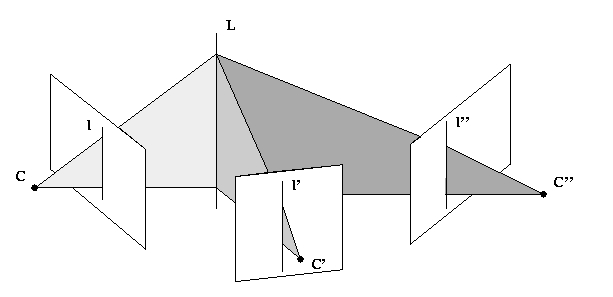
\includegraphics[width=.45\textwidth]{figures/threeviews.jpg}
 }\\
 Let the Camera positions be $C_{c^*},C_c,C_i$ for the desired, current, and initial camera positions respectively. And their projection matrices are $[I | 0]$, $[ ^{c}{\bf R}_{c^*} | ^{c}{\bf t}_{c^*} ]$, $[ ^{i}{\bf R}_{c^*} | ^{i}{\bf t}_{c^*} ]$. The Tensor relationfor calibrated cameras can then be expressed as follows:
$$
\mathcal{T}_{(jkl)} = \tensor[^{c}]{R}{_{c^{*}(kj)}} \ \tensor[^{i}]{t}{_{c^{*}(l)}} - \tensor[^{c}]{t}{_{c^{*}(k)}} \ \tensor[^{i}]{R}{_{c^{*}(lj)}}
$$
The trifocal tensor can be computed from feature correspondences across the three views \cite{Hartley2004}. Each triplet of corresponding image points gives 4 equations linearly independent. Therefore, a minimum set of 7 correspondences of points are needed for the trifocal tensor computation to uniquely determine the 27 entries of the tensor matrix.
  \end{multicols}
}{
Visual servoing is an approach for controlling the motion of a robotic system from visual measurements \cite{chaumette2006visual}. The trifocal tensor is well known in computer vision for tracing geometric information from three images of the same scene \cite{Hartley2004}.  The trifocal tensor geometric model is more robust than the two view geometry models as it involves the information given by a third view, and the set of correspondences obtained is more robust to outliers.
{\centering 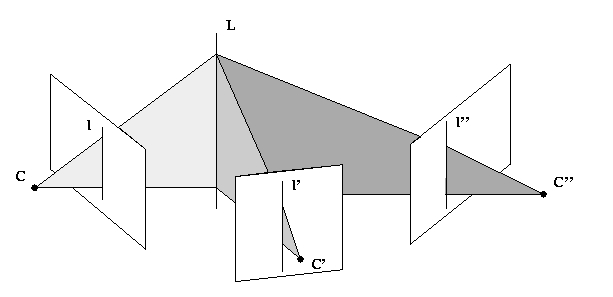
\includegraphics[width=.9\textwidth]{figures/threeviews.jpg}
}\\
Let the camera positions be $C_{c^*},C_c,C_i$ for the desired, current, and initial camera positions respectively, and their projection matrices be $[I | 0]$, $[ ^{c}{\bf R}_{c^*} | ^{c}{\bf t}_{c^*} ]$, $[ ^{i}{\bf R}_{c^*} | ^{i}{\bf t}_{c^*} ]$. The Tensor relation for calibrated cameras can then be expressed as follows:
$$
\mathcal{T}_{(jkl)} = \tensor[^{c}]{R}{_{c^{*}(kj)}} \ \tensor[^{i}]{t}{_{c^{*}(l)}} - \tensor[^{c}]{t}{_{c^{*}(k)}} \ \tensor[^{i}]{R}{_{c^{*}(lj)}}
$$
The trifocal tensor can be computed from feature correspondences across the three views up to a scale factor \cite{Hartley2004}. Each triplet of corresponding image points gives 4 equations linearly independent. Therefore, a minimum set of 7 correspondences of non-planar points are needed for the trifocal tensor computation to uniquely determine the 27 entries of the tensor matrix.
}

 }

%%%%%%%%%%%%%%%%%%%%%%%%%%%%%%%%%%%%%%%%%%%%%%%%%%%%%%%%%%%%%%%%%%%%%%%%%%%%%%
  \headerbox{3. Methodology}{name=methodology,column=0,span=2,row=1,below=definition}{
%%%%%%%%%%%%%%%%%%%%%%%%%%%%%%%%%%%%%%%%%%%%%%%%%%%%%%%%%%%%%%%%%%%%%%%%%%%%%%
    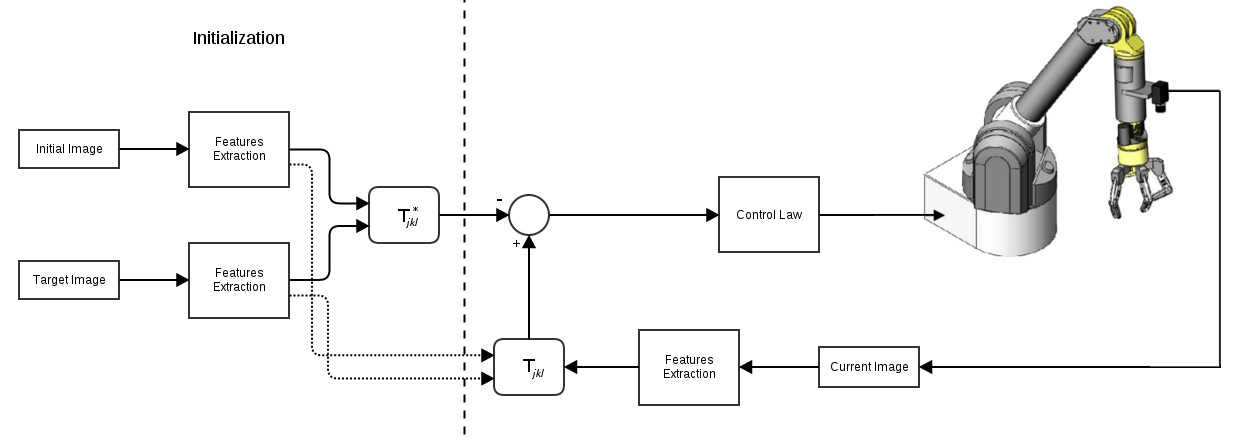
\includegraphics[width=.9\textwidth,height=40mm]{figures/vsttloop.png}
\begin{multicols}{2}
  Since the trifocal tensor is computed up to a scale factor, we propose a normalization step to get a fixed scale. The normaliztion factors $\mathcal{T}_{kN}$ are used to obtain the normalized tensor $T_{jkl}$.
\begin{gather*}
  T_{jkl} = \frac{\mathcal{T}_{jkl}}{\mathcal{T}_{kN}}, \mathcal{T}_{kN} = (\sum_n \sum_m {\mathcal{T}_{nkm}}^{2}) ^{\frac{1}{2}}
\end{gather*}
The derivation of the normalized trifocal tensor corresponding interaction matrix $L_{T_{(jkl)}}$ is then:
\begin{align*}
  \dot{T}_{(jkl)} &= L_{T_{(jkl)}} u_c\\
                  &= \frac{\textcolor{lightblue}{\tensor[^{i}]{R}{_{c^{*}(lj)}}}}{\mathcal{T}_{kN}}v_{c(k)} +\sum_{m} {[\omega_{c}]}_{\times(km)} T_{(jml)}\\&-T_{(jkl)}(\sum_n \sum_{m}T_{nkm}\frac{ \textcolor{lightblue}{\tensor[^{i}]{R}{_{c^{*}(mn)}}} }{\mathcal{T}_{kN}}) v_{c(k)} \\&+ T_{(jkl)}(\sum_n \sum_{m}T_{nkm}T_{nhm})\omega_{(g)} \\&- T_{(jkl)}(\sum_n \sum_{m}T_{nkm}T_{ngm})\omega_{(h)}\\
  \text{where } g &= k\%3 +1, h = (k+1)\%3 +1
  \end{align*}
With all elements defined, the control law is computed, and the visual servoing task is as follows:
\begin{gather*}
    e = T_{(jkl)} - T_{(jkl)}^{*}\\
  u_c = -\lambda L_{T_{(jkl)}}^{+} e
\end{gather*}
\begin{enumerate}\compresslist
  \item At initialization, the desired tensor $T_{(jkl)}^{*}$ is computed from feature correspondences across the three images.
  \item The current tensor $T_{(jkl)}$ is computed inside the visual servoing loop at each iteration.
  \item The interaction matrix $L_{T_{(jkl)}}$ is computed using the current tensor.
  \item The required velocities to drive the camera to the desired pose are computed with the new error value and the pseudo-inverse of the interaction matrix.
  \item The system converges and the loop is terminated when the camera reaches the desired pose, means the error value is less than a defined threshold.
\end{enumerate}
\end{multicols}

}

%%%%%%%%%%%%%%%%%%%%%%%%%%%%%%%%%%%%%%%%%%%%%%%%%%%%%%%%%%%%%%%%%%%%%%%%%%%%%%
\headerbox{2. Contributions}{name=contributions,column=2,row=0}{
  An approach to incorporate the trifocal tensor estimated from the calibrated three-view geometry into the visual servoing control loop task is proposed. This approach presents a generalized 6-DOF visual servoing task, with the control loop being closed over projective measures, namely the trifocal tensor coefficients. To the best of our knowledge, this approach is the first to propose a fully analytical design for a 6-DOF visual servoing task based on the trifocal tensor \cite{lopez2010visual}\cite{shademan2010three}.

}

%%%%%%%%%%%%%%%%%%%%%%%%%%%%%%%%%%%%%%%%%%%%%%%%%%%%%%%%%%%%%%%%%%%%%%%%%%%%%%
\headerbox{4. Results}{name=results,column=2,below=contributions}{
  \iftoggle{portrait}{
\vfill
  \begin{center}
  \begin{tabular}{cc}
  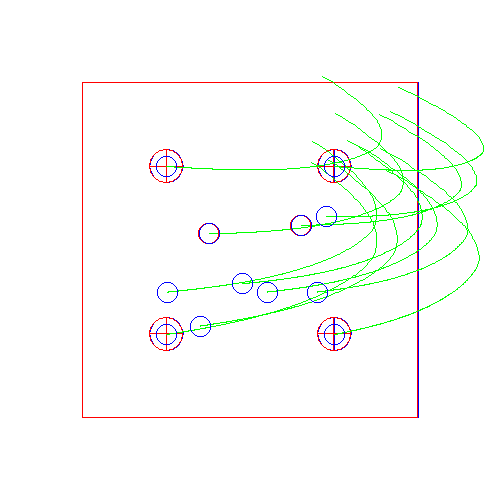
\includegraphics[height=0.1\textheight]{figures/plots/ex5cimage.png}&
  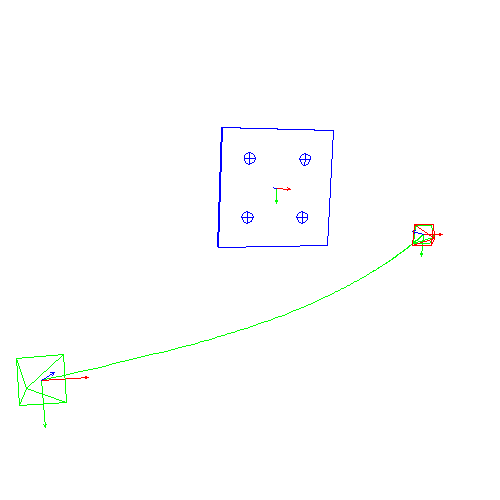
\includegraphics[height=0.1\textheight]{figures/plots/ex5cscene.png}\\
  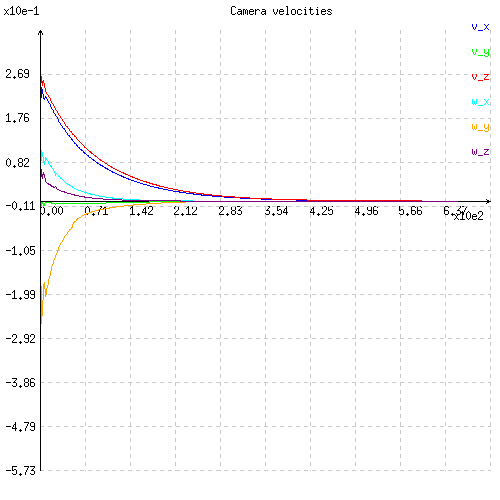
\includegraphics[height=0.1\textheight]{figures/plots/ex5cvelocity.png}&
  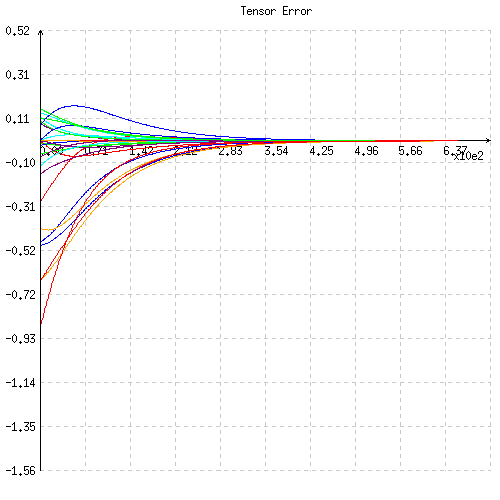
\includegraphics[height=0.1\textheight]{figures/plots/ex5cerror.png}\\
  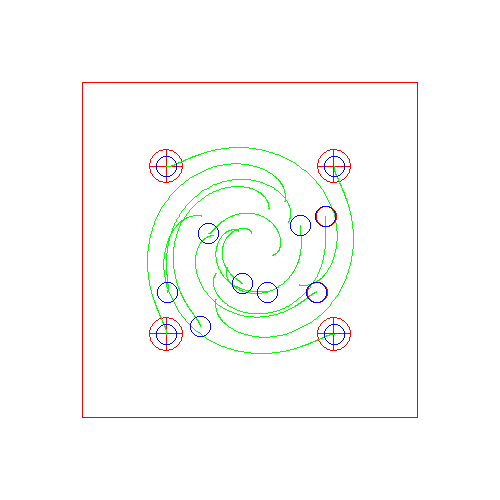
\includegraphics[height=0.1\textheight]{figures/plots/ex4cimage.png}&
  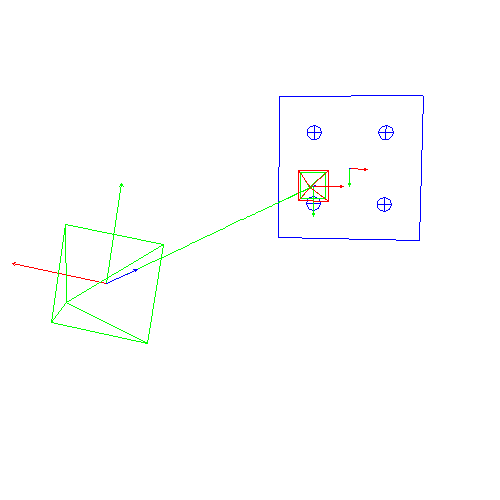
\includegraphics[height=0.1\textheight]{figures/plots/ex4cscene.png}\\
  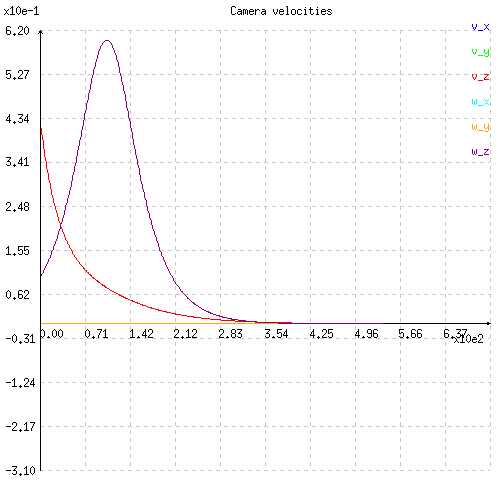
\includegraphics[height=0.1\textheight]{figures/plots/ex4cvelocity.png}&
  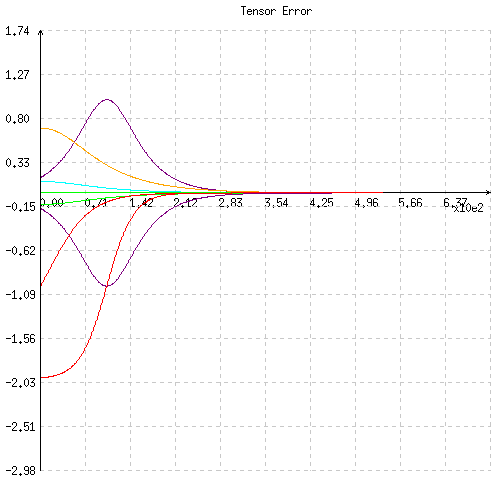
\includegraphics[height=0.1\textheight]{figures/plots/ex4cerror.png}\\
  \end{tabular}
  \end{center}
\vfill
}{
\vfill
\begin{center}
  \begin{tabular}{cc}
  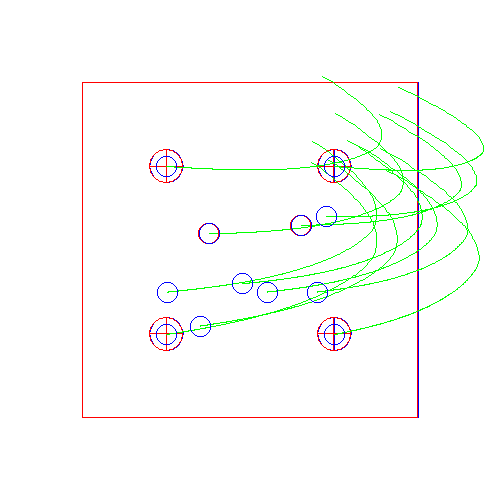
\includegraphics[height=0.15\textheight]{figures/plots/ex5cimage.png}&
  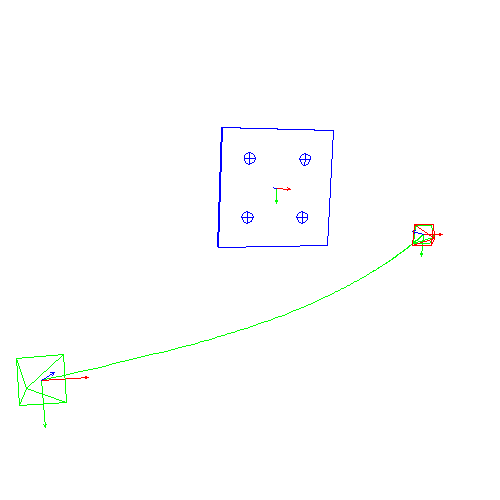
\includegraphics[height=0.15\textheight]{figures/plots/ex5cscene.png}\\
  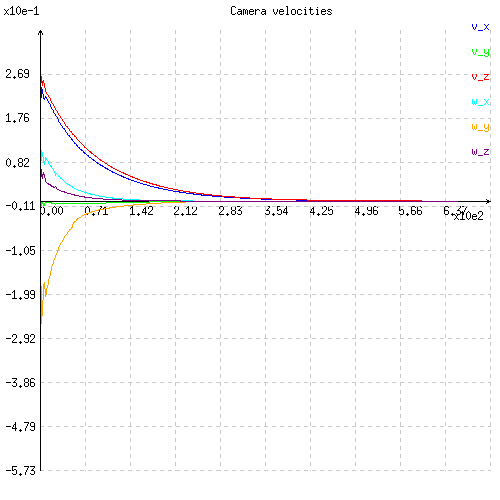
\includegraphics[height=0.15\textheight]{figures/plots/ex5cvelocity.png}&
  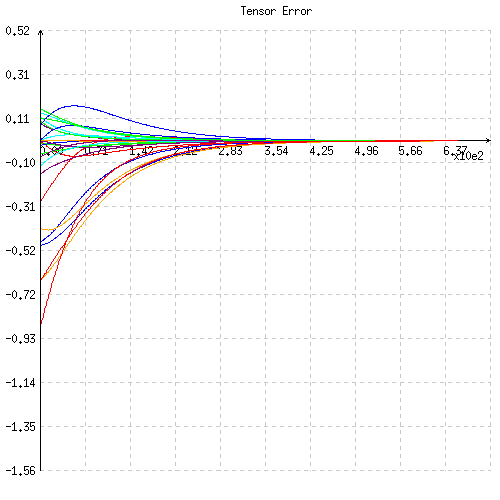
\includegraphics[height=0.15\textheight]{figures/plots/ex5cerror.png}\\
  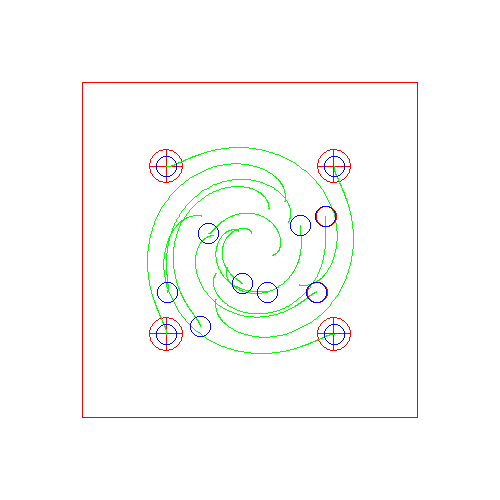
\includegraphics[height=0.15\textheight]{figures/plots/ex4cimage.png}&
  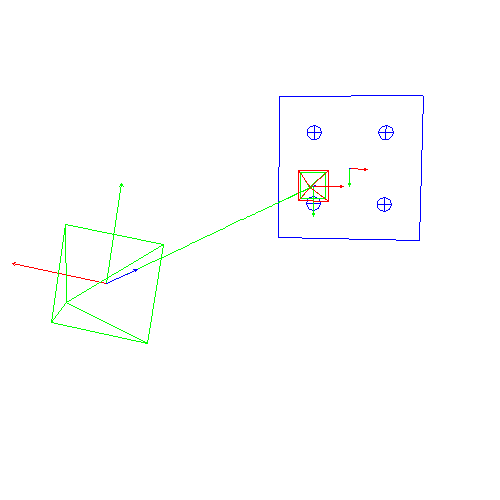
\includegraphics[height=0.15\textheight]{figures/plots/ex4cscene.png}\\
  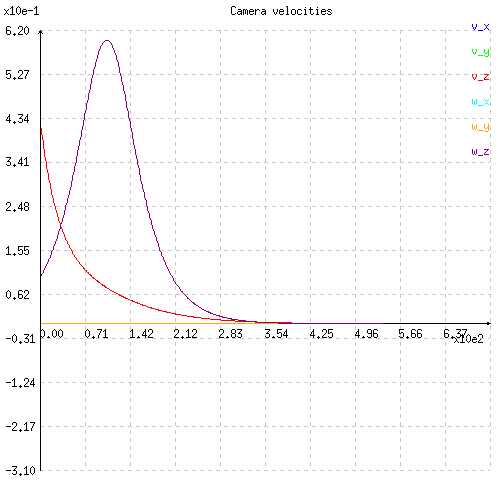
\includegraphics[height=0.15\textheight]{figures/plots/ex4cvelocity.png}&
  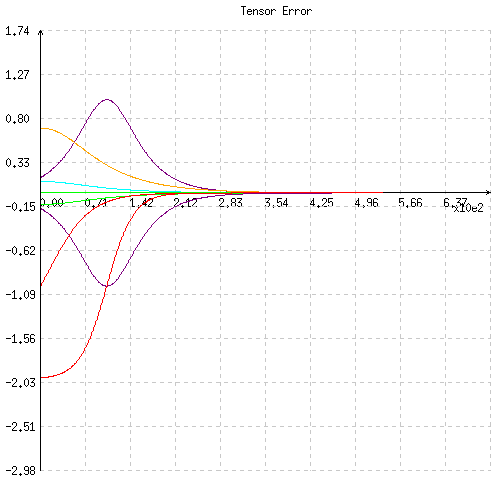
\includegraphics[height=0.15\textheight]{figures/plots/ex4cerror.png}\\
  \end{tabular}
\end{center}
\vfill
}
\begin{enumerate}\compresslist
  \item The approach is working practically with very satisfactory results.
  \item Does not suffer from some of the problems existing in IBVS methods namely the retreat problem.
  \item In the interaction matrix, we have a decoupling between the translational velocities, means smooth camera trajectories for the motion in the 3D space.
\end{enumerate}
However, the \textcolor{lightblue}{initial rotation matrix} is a parameter that needs to be estimated.

}
%%%%%%%%%%%%%%%%%%%%%%%%%%%%%%%%%%%%%%%%%%%%%%%%%%%%%%%%%%%%%%%%%%%%%%%%%%%%%%
%%%%%%%%%%%%%%%%%%%%%%%%%%%%%%%%%%%%%%%%%%%%%%%%%%%%%%%%%%%%%%%%%%%%%%%%%%%%%%
%\headerbox{4. Motion estimation}{name=motion,column=1,below=bgtrack}{

%}

%%%%%%%%%%%%%%%%%%%%%%%%%%%%%%%%%%%%%%%%%%%%%%%%%%%%%%%%%%%%%%%%%%%%%%%%%%%%%%
  %\headerbox{7. Contributions}{name=contribution,column=3,row=0,below=Applications}{

   %Our main contributions are
   %\begin{enumerate}\compresslist
   %\item A method to compute superpixel matchings (The superpixel flow).
   %\item A segmentation method for objects in video (Background regions tracking).
   %\item A framework to combine object trackers and optical flow methods.
   %\item A method to extend the Simple Flow method to use input segmentation masks.
   %\item A better sampling method for tracking-by-detection methods.

   %\end{enumerate}
   %%\vspace{0.3em}
  %}
%%%%%%%%%%%%%%%%%%%%%%%%%%%%%%%%%%%%%%%%%%%%%%%%%%%%%%%%%%%%%%%%%%%%%%%%%%%%%%
  \headerbox{5. Bibliography}{name=bibliography,column=0,span=2,below=methodology}{

    \bibliographystyle{IEEEtran}
    \renewcommand{\section}[2]{\vskip 0.05em}
    %\nocite{*}
    \bibliography{tex/refs}
%\bibliographystyle{ieee}
      %\begin{thebibliography}{1}\itemsep=-0.01em
      %\setlength{\baselineskip}{0.4em}

      %\bibitem{c1}
      %M. Tao, J. Bai, P. Kohli, and S. Paris. SimpleFlow: A Non-iterative, Sublinear Optical Flow Algorithm, {\it Eurographics '12}

      %\bibitem{c2}
      %S. Baker, D. Scharstein, J.P. Lewis, S. Roth, M.J. Black and R. Szeliski. A Database and Evaluation Methodology for Optical Flow, {\it IJCV '13}

      %\bibitem{c3}
      %Y. Boykov, M-P. Jolly. Interactive Graph Cuts for Optimal Boundary \& Region Segmentation of Objects in N-D images, {\it ICCV '13}

      %\bibitem{c4}
      %Y. Wu, J. Lim and M.-H. Yang. Online object tracking: A benchmark, {\it CVPR '13}

      %\end{thebibliography}

   %%\vspace{0.3em}
  }

\end{poster}

\end{document}
